\documentclass[10pt]{article}
\usepackage[utf8]{inputenc}
\usepackage[T1]{fontenc}
\usepackage{amsmath}
\usepackage{amsfonts}
\usepackage{amssymb}
\usepackage[version=4]{mhchem}
\usepackage{stmaryrd}
\usepackage{graphicx}
\usepackage[export]{adjustbox}
\graphicspath{ {./images/} }

\title{Measurement of scintillating fibres for the LHCb experiment }

\author{Can Toraman\\
can.toraman@tu-dortmund.de}
\date{}


\begin{document}
\maketitle
Measurements: 03.05.2024\\
Hand-in: 21.05.2024

\section*{Contents}
1 Objective 3\\
2 Theory 3\\
2.1 Scintilating fiber trackers . . . . . . . . . . . . . . . . . . . . . . . . . . . 3\\
2.2 Scintillating fibers . . . . . . . . . . . . . . . . . . . . . . . . . . . . . . . 4\\
2.2.1 Structure of scintillating fibers . . . . . . . . . . . . . . . . . . . . 4\\
2.2.2 Photon propagation in the fibers . . . . . . . . . . . . . . . . . . . 5

3 Experimental setup 7

\begin{center}
\begin{tabular}{|ll|}
\hline
4 Measuring tasks & $\mathbf{7}$ \\
\hline
\end{tabular}
\end{center}

4.1 Spectrometer measurement . . . . . . . . . . . . . . . . . . . . . . . . . . 8\\
4.2 Radial symmetry . . . . . . . . . . . . . . . . . . . . . . . . . . . . . . . . 8\\
4.3 Intensity measurement . . . . . . . . . . . . . . . . . . . . . . . . . . . . . 8\\
4.4 Angle intensity measurement . . . . . . . . . . . . . . . . . . . . . . . . . 8

5 Analysis 9\\
5.1 Spectrometer measurement . . . . . . . . . . . . . . . . . . . . . . . . . . 9\\
5.2 Radial symmetry measurement . . . . . . . . . . . . . . . . . . . . . . . . 10

5 . Simulation . . . . . . . . . . . . . . . . . . . . . . . . . . . . . . . . . . . . 10\\
5.3.1 Simulation cleaning . . . . . . . . . . . . . . . . . . . . . . . . . . 10\\
5.3.2 Production angle . . . . . . . . . . . . . . . . . . . . . . . . . . . . 11\\
5.3.3 Minimum distance . . . . . . . . . . . . . . . . . . . . . . . . . . . 12\\
5.3.4 Intensity. . . . . . . . . . . . . . . . . . . . . . . . . . . . . . . . . 13\\
5.4 Intensity measurement . . . . . . . . . . . . . . . . . . . . . . . . . . . . . 14\\
5.5 Angle Intensity Measurement . . . . . . . . . . . . . . . . . . . . . . . . . 16

6 Discussion 17\\
References 18

\section*{1 Objective}
The objective of this lab course is to understand the basic concepts of scintillating fibers. This is achieved by measuring different aspects of the light propagation inside the fibers and comparing the results with simulated data.

\section*{2 Theory}
In detectors for high energy particle physics, a precise track reconstruction is crucial to succefully analyse collision events. There are many different solutions to realising such a tracking detector, each with their own advantages and disadvantages, for example in regard to their resolution, size, cost. Tracking devices using scintillators are one type of such a detector, an example of their application is the famous LHCb experiment. If charged particles pass through a scintillator, photons are emmited that can be measured. The following section will explain how a tracking detector can be constructed using this principle.

\subsection*{2.1 Scintilating fiber trackers}
A tracker is constructed by using many individual scintillating fibers. If a charged particle passes through one of these fibers, photons are produced that travel towards the end of the fiber, where they can be detected. The main advantages of this type of tracker is its high resolution, as the fibers can be constructed rather thin ( $250 \mu \mathrm{~m}$ in LHCb ). As the probability of a single fiber being hit by a charged particle can be decribed by a uniform distribution, the resolution of a fiber of width $d$ can be calculated using the standard deviation of this distribution:

$$
\sigma_{\text {fiber }}=\sqrt{\frac{d^{2}}{12}} .
$$

Inserting the given width of $250 \mu \mathrm{~m}$, a resolution of $\approx 72 \mu \mathrm{~m}$ results. Penetrating particles are scattered less in the fibers compared to other methods, consequently the error introduced by the detector is kept low. Lastly, these fibers are inexpensive meaning a large surface can be covered, this increases the total amount of particles that can be measured by the detector [1]. The single fibers are combined into fiber mats, by arranging them in a hexagonal pattern to minimize uncovered area and glueing them together using an epoxy. A cross section of this arrangment can be seen in Figure 1.\\
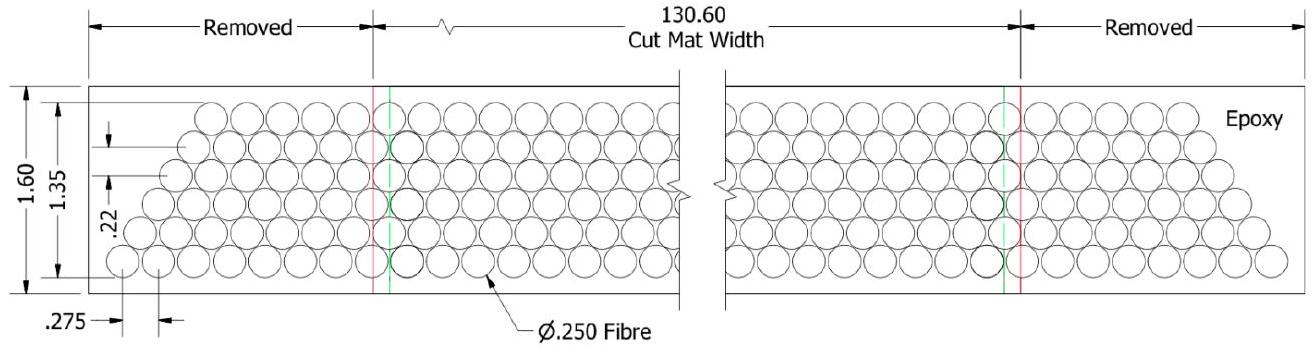
\includegraphics[max width=\textwidth, center]{2025_06_26_8f443d40fa1f5ba53fc3g-04}

Figure 1: Cross section of the fiber mat constructed out of the scintillating fibers $[1]$.

In case of the LHCb detector four layers, each consisting of 40 mats, are positioned behind each other. The middle layers are tilted by $\pm 5^{\circ}$ to allow a spacial resolution in the entire plane perpendicular to the beam pipe. There are three individual tracking stations constructed in this way.\\
The photons created by the scintillations travel to the ends of the fibers and are detected there using silicon photomultipliers. These consit of avalanche photodiodes, where each diode represents a pixel. If a photon hits a pixel, an electron-hole pair is created in the diode. Due to an applied high voltage, the electrons are accelerated and trigger more electron-hole pairs to form. Consequentlly, a charge avalanche is registered in form of a current pulse. After a short recovery time, the pixel is ready to sense another signal. The silicon photomultipliers cannot detect all incoming photons, they have a photodetection efficiency depending on the wavelength of the photons. At the optimal wavelength, a maximum of $43 \%$ of photons can be detected. The silicon photomultipliers themselves are not sensitive to the wavelength of the light and thus measure an effective attenuation over all wavelengths. Lastly, there will always be a certain noise within the pixels leading to the presence of a dark current, even if no photons hit the pixel.

\subsection*{2.2 Scintillating fibers}
In the following, the internal structure of the scintillating fibers will be explained. Additionally, some important explainations about how the light propagates inside the fibers are given.

\subsection*{2.2.1 Structure of scintillating fibers}
The center of the fibers consits of a $220 \mu \mathrm{~m}$ thick polystyrene core. This is an organic scintillator, meaning that the scintillations caused by charged particles are based on molecular processes. If a charged particle passes through the fiber, valence electrons of the polystyrene are excited. During the relaxation process, UV photons are emmited and travel through the fiber. To ensure that the photons remain inside the fiber, the outer layers are chosen in a way to allow total internal reflection to occur. This is archieved by surrounding the core with two sheats with outwardly decreasing refractive indices. Both sheats have a thickness of $7.5 \mu \mathrm{~m}$, resulting in a total fiber width of $250 \mu \mathrm{~m}$. A basic sktech of this fiber layout can be seen in Figure 2.\\
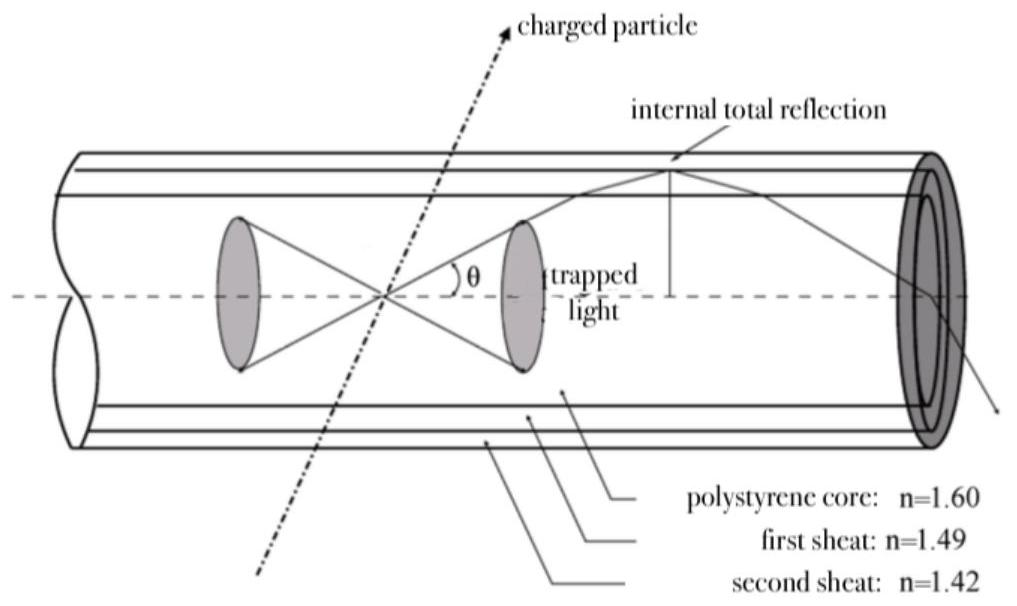
\includegraphics[max width=\textwidth, center]{2025_06_26_8f443d40fa1f5ba53fc3g-05(1)}

Figure 2: Schematic structure of the scintillating fiber used in the experiment [1].

The refractive indices are also given in Figure 2, it can easily be seen that they decrease towards the outside of the fiber. This ensures proper propagation of the photons discussed in the next chapter.

\subsection*{2.2.2 Photon propagation in the fibers}
Since the UV photons will always be emmited at a certain distance from the center of the fiber and with a given angle $\theta$, reflections at the first and second sheat will occur. This is visualized in Figure 3. During its path, the photon will have a minimal distance $r_{\text {min }}$ from the center of the fiber.\\
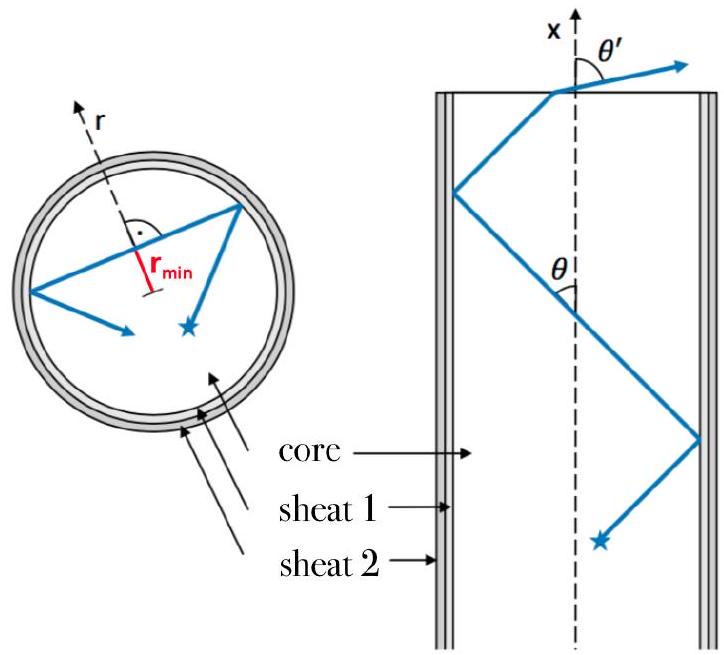
\includegraphics[max width=\textwidth, center]{2025_06_26_8f443d40fa1f5ba53fc3g-05}

Figure 3: Path of a photon trough the scintillating fiber 1 .

Assuming that the photon remains inside the core, the path length of the photon $L$ and\\
the number of times it reflects $N$ are given by


\begin{align*}
L & =\frac{x}{\cos \theta}  \tag{1}\\
N & =\frac{x \tan \theta}{2 \sqrt{r_{\text {core }}^{2}-r_{\text {min }}^{2}}} \tag{2}
\end{align*}


Here, $r_{\text {core }}$ is the radius of the fiber core and $x$ is the distance to the fiber end. The angle towards the inteface $\theta_{\text {refl }}$ at the end of the fiber can be calculated using the formula

$$
\theta_{\mathrm{refl}}=\arcsin \left(\sqrt{1-\frac{r_{\mathrm{min}}^{2}}{r_{\mathrm{core}}^{2}}} \sin \theta\right)
$$

Some of the photons travelling inside the fiber are lost due to different processes. This is why the fiber has a specific capture efficiency that describes what fraction of photons remain inside it. Photons can undergo Raygleigh scattering with the fiber material or be absorbed by it. In general, the attentuation $I$ of photons after traveling a distance $L$ in the fiber exponentially decreases according to


\begin{equation*}
I(x)=I_{0} \exp \left(-\frac{L}{\Lambda}\right)=I_{0} \exp (-a L) \tag{3}
\end{equation*}


where $\Lambda$ is the attentuation length which is approximatly 3.5 m in the fibers used for this experiment. The inverse attentuation length $a$ is called the attenuation coefficient. To further parameterize the photon attentuation, it is useful to differentiate between losses due to the core material $A_{\text {core }}$ and losses due to reflection $A_{\text {refl }}$. Now the total attentuation can be expressed as


\begin{equation*}
I(x, \theta)=I_{0} A_{\text {core }}(x, \theta) A_{\text {refl }}(x, \theta) . \tag{4}
\end{equation*}


Losses in the core material depend exponentially on the path length of the photon via


\begin{equation*}
A_{\text {core }}(x, \theta)=\exp \left(-\frac{L(x, \theta)}{\Lambda}\right) \tag{5}
\end{equation*}


For reflection losses, the number of reflections $N$ and probability of loss during reflection $\varepsilon$ is needed. In this case, the losses also show an exponential dependance on these parameters:


\begin{equation*}
A_{\mathrm{refl}}(x, \theta)=\exp (-\varepsilon N(x, \theta)) \tag{6}
\end{equation*}


Now, relations (5) and (6) can be inserted into (4). Lastly, the known expressions for $L(x, \theta)$ (1) and $N(x, \theta)$ (2) can be used to obtain the final formula


\begin{equation*}
I(x, \theta)=I_{0} \exp (-x \underbrace{\left(\frac{1}{\cos \theta}+\frac{\varepsilon \tan \theta}{2 \sqrt{r_{\mathrm{core}}^{2}-r_{\mathrm{min}}^{2}}}\right)}_{a_{\mathrm{eff}}}) \tag{7}
\end{equation*}


Here, $a_{\text {eff }}$ summarizes the parameters as the effective attentuation coefficient.

\section*{3 Experimental setup}
The experiment consits of a single scintillating fiber, which can be excited using a LED. A picure of the setup can be seen in Figure 4.\\
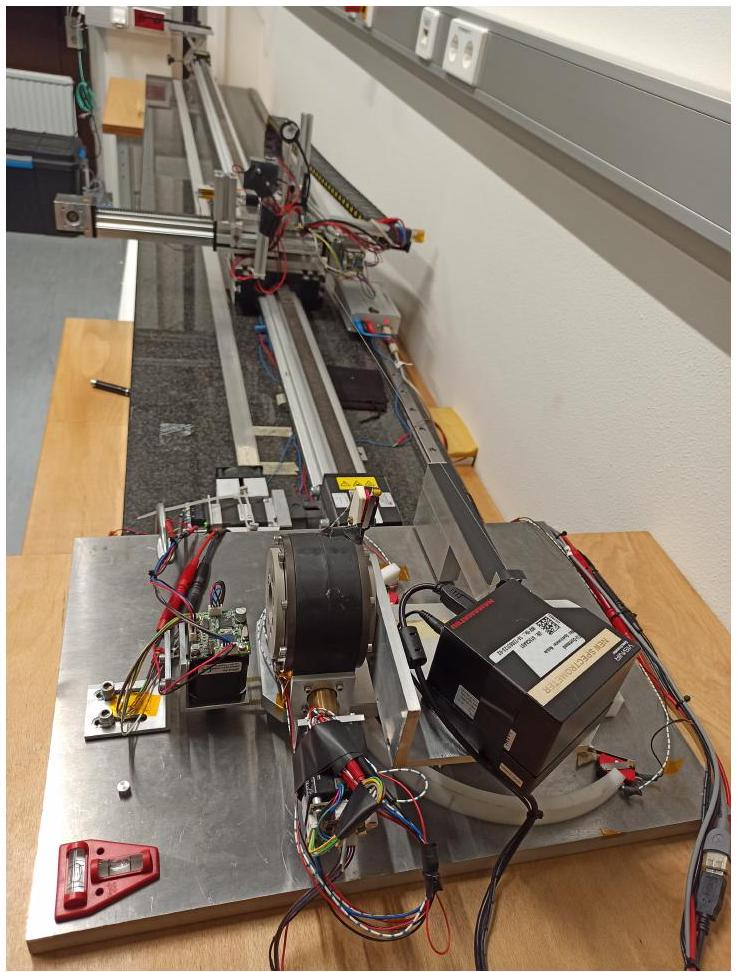
\includegraphics[max width=\textwidth, center]{2025_06_26_8f443d40fa1f5ba53fc3g-07}

Figure 4: Experimental setup consisting of the fiber, the LED and spectrometer.

The LED can be moved along the fiber to be able to excite it at different positions. At one end of the fiber, a spectrometer is positioned. It can be tilted in the horizontal and vertical plane within the angle intervals $\left[-20^{\circ}, 90^{\circ}\right]$ and $\left[-6^{\circ}, 90^{\circ}\right]$, respectively. The entire setup is connected to a computer, which runs a programm that allows to set all paramters for a measurement. The simulation data needed for the analysis is already produced with Geant4. Here, 50 fibers were excited and simulated at 24 points each.

\section*{4 Measuring tasks}
For every measurement, the dark counts are also saved. These are the counts that are measured by the spectrometer even if the LED is turned of and the fiber is not excited. In the analysis, these will be substracted from the actual counts to remove the effect of the dark current. The current of the LED is always set to 20 mA . The same holds for the integration time and number of averages, which are $10000 \mu \mathrm{~s}$ and 5 in all measurements, respectively.

\subsection*{4.1 Spectrometer measurement}
The first measurement is taken without varying the excitation position or the spectrometer angle. Instead, the wavelength dependance of the emmited photon intensity is measured by the spectrometer. This is done with the room light on and room light off, the two results are later compared.

\subsection*{4.2 Radial symmetry}
Now, the horizontal and vertical angle of the spectrometer are varied, while the excitation position is kept constant. The angle intervall tested is $\left[-18^{\circ}, 30^{\circ}\right]$ in the horizontal plane and $\left[-6^{\circ}, 35^{\circ}\right]$ in the vertical plane. In both cases, 15 values are taken, resulting in a total of 225 data points.

\subsection*{4.3 Intensity measurement}
The dependancy of the light intensity on the distance is measured by altering the excitation location of the fiber. The fiber is excited in an interval of 150 cm , where the LED is moved in 7.5 cm increments. For each LED position, 10 different horizontal angles in the interval $\left[0^{\circ}, 40^{\circ}\right]$ are measured. A defective spot in the fiber was visible when exciting it, its effect will be taken into account during the analysis.

\subsection*{4.4 Angle intensity measurement}
For the last measurement, the excitation position is kept constant again. The fiber is excited and only the horizontal position of the spectrometer is varied in the interval $\left[0^{\circ}, 45^{\circ}\right] .90$ data points are taken by choosing $0.5^{\circ}$ steps between the measurements.

\section*{5 Analysis}
\subsection*{5.1 Spectrometer measurement}
Initially, the two measurements of the spectra are plotted and shown in Figure 5. These show the effect the roomlight has on a measurement.\\
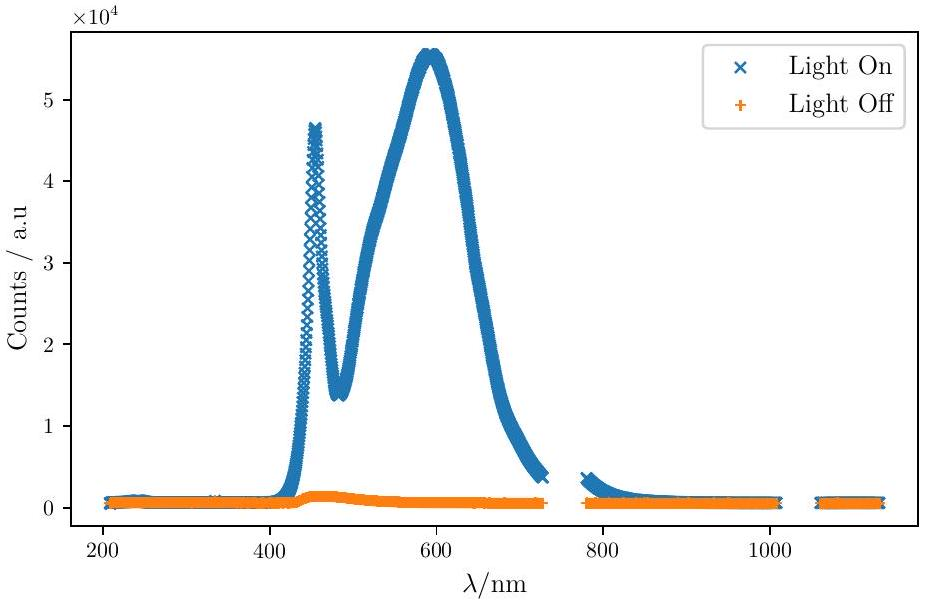
\includegraphics[max width=\textwidth, center]{2025_06_26_8f443d40fa1f5ba53fc3g-09}

Figure 5: Recorded wavelength spectra and their respective counts at a fixed distance and fixed angles.

To reduce the effect of external light sources, the counts during a measurement with the led activated are subtracted by the dark counts (measurements with the laser deactivated). The newly cleaned spectra are shown in Figure 6.\\
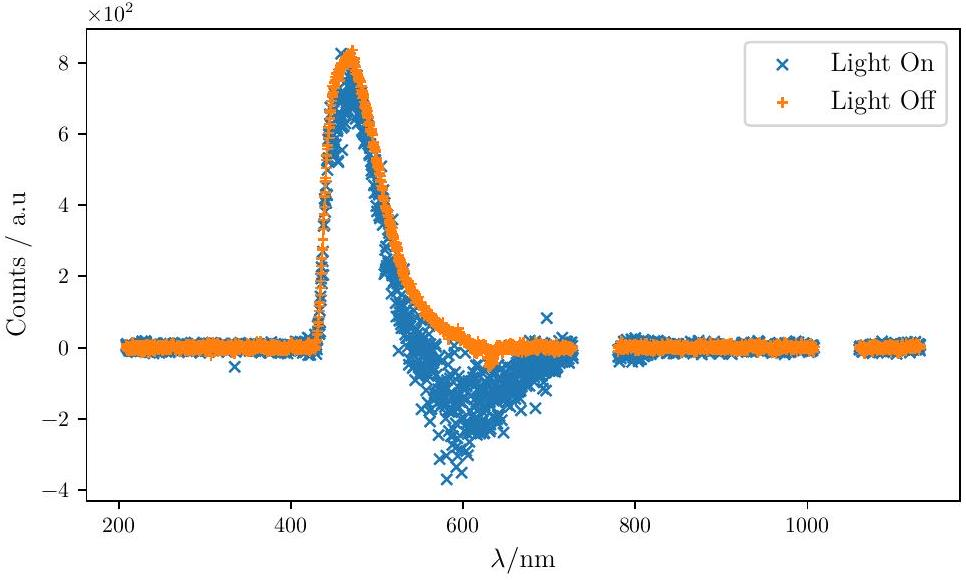
\includegraphics[max width=\textwidth, center]{2025_06_26_8f443d40fa1f5ba53fc3g-09(1)}

Figure 6: Wavelength spectra and their respective counts with the dark counts removed.

\subsection*{5.2 Radial symmetry measurement}
The goal of this part of the analysis is the visualization of the light intensity in relation to the horizontal and vertical measurement angles. The intensity is determined as the sum of the counts of a measured spectrum with the dark counts subtracted. Additionally, each intensity is normed via dividing by the highest measured intensity. The results are plotted in a two-dimensional histogram shown in Figure 7.\\
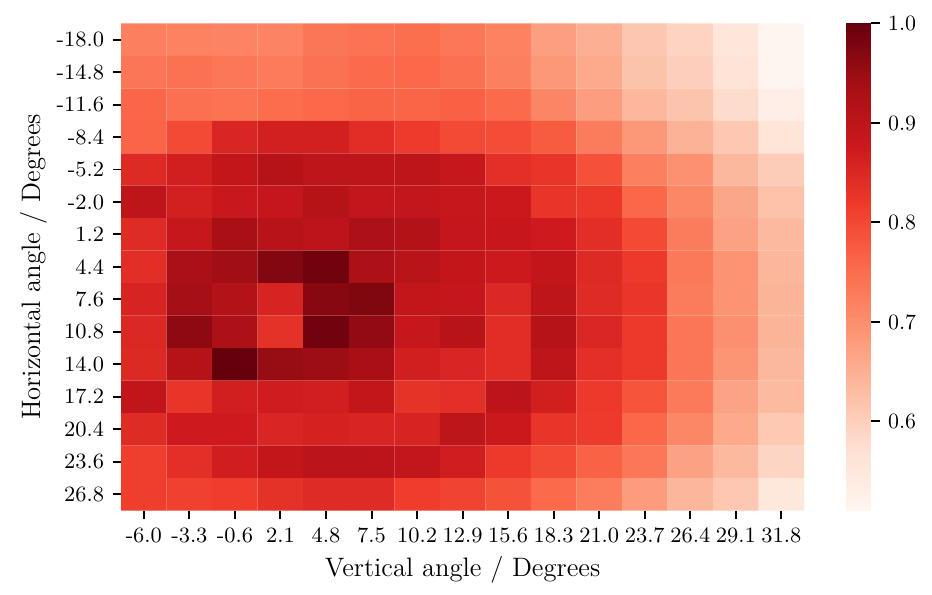
\includegraphics[max width=\textwidth, center]{2025_06_26_8f443d40fa1f5ba53fc3g-10}

Figure 7: Angular distribution of the measured intensity in relation the horizontal and vertical angle.

\subsection*{5.3 Simulation}
The simulated data is created using the software GEANT4 and consists of 1200 Files with 14 features each. These are used to better understand the photon propagation in the fiber.

\subsection*{5.3.1 Simulation cleaning}
Due to errors in the simulation process, some of the generated events have to be removed. This includes photons arriving at the photomultiplier outside of the fiber as well as photons that underwent Rayleigh scattering. The effect of the wrongly generated events and the application of a requirement on the calculated r\_exit variable (distance to the core of the fiber) r\_exit $\leq 0.125 \mathrm{~mm}$ is shown in Figure 8.\\
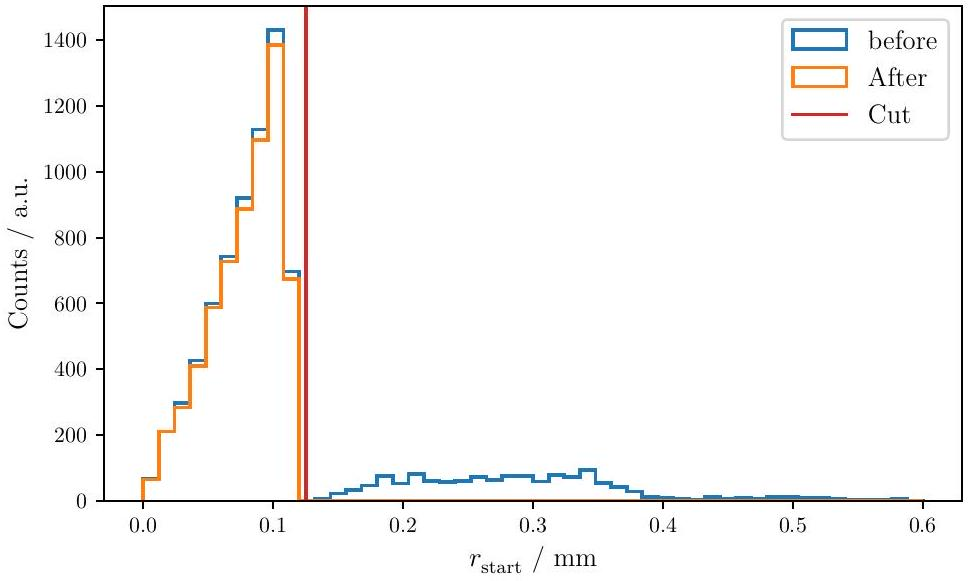
\includegraphics[max width=\textwidth, center]{2025_06_26_8f443d40fa1f5ba53fc3g-11}

Figure 8: Distribution of the exit distances $r_{\text {min }}$ in the simulation sample before and after the applied requirement (red line).

Additionally, the simulation data is split into two samples for core and cladding photons. Measurements of core photons have a length\_clad $=0$ and cladding photons length\_clad $\neq 0$.

\subsection*{5.3.2 Production angle}
Initially the maximum angles for which internal reflection can occur are determined using the formulas

$$
\begin{aligned}
& \theta_{1}=\arccos \left(\frac{n_{2}}{n_{1}}\right)=21.37^{\circ} \text { and } \\
& \theta_{2}=\arccos \left(\frac{n_{3}}{n_{1}}\right)=27.44^{\circ}
\end{aligned}
$$

where $n_{1}, n_{2}$, and $n_{3}$ are the refraction indices inside the scintillating fiber. Following the aforementioned step, the angles $\theta$ of the simulation data have to be determined by calculating the angle between the momentum of the generated photon and the $x$-axis. The histogrammed angles of both simulation data samples are shown in Figure 9 along the two theoretically determined angles.\\
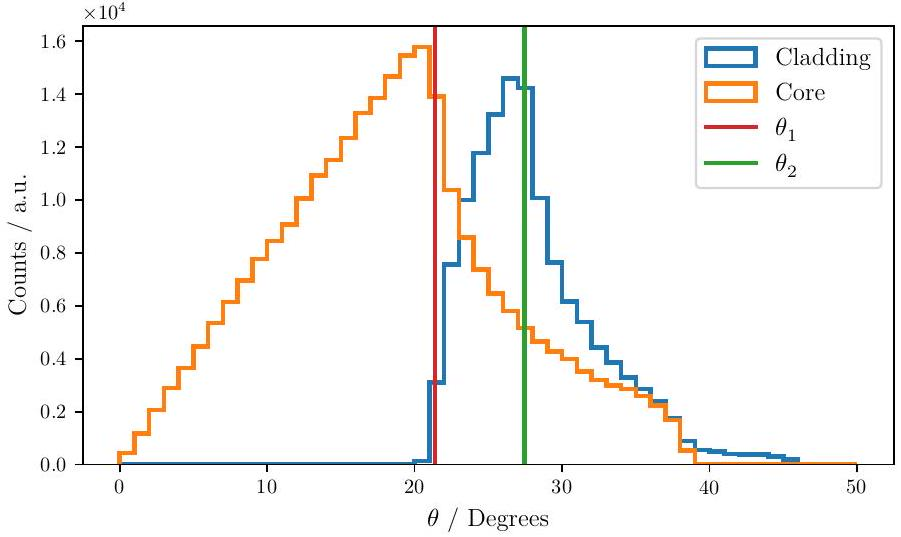
\includegraphics[max width=\textwidth, center]{2025_06_26_8f443d40fa1f5ba53fc3g-12}

Figure 9: Angular distribution for both the core and cladding photons and the calculated maximum angles $\theta_{1}$ and $\theta_{2}$.

\subsection*{5.3.3 Minimum distance}
The minimum distance between the path of the photon and the $x$-axis is calculated using the formula

$$
r_{\min }=\left|\frac{z * p_{y}-p_{z} y}{\sqrt{p_{z}^{2}+p_{y}^{2}}}\right|,
$$

where $y, z, p_{y}$, and $p_{z}$ are the positions and momenta of the photon at its starting point. This formula is obtained by calculating the minimal distance of the photons path (starting point $x, y, z$ and direction $p_{x}, p_{y}, p_{z}$ ) from the $x$-axis. Using this newly created variable and the already determined production angle, a two-dimensional histogram is created to visualize their relation. The histogram for the core photons is shown in Figure 10a and for the cladding photons in Figure 10b.\\
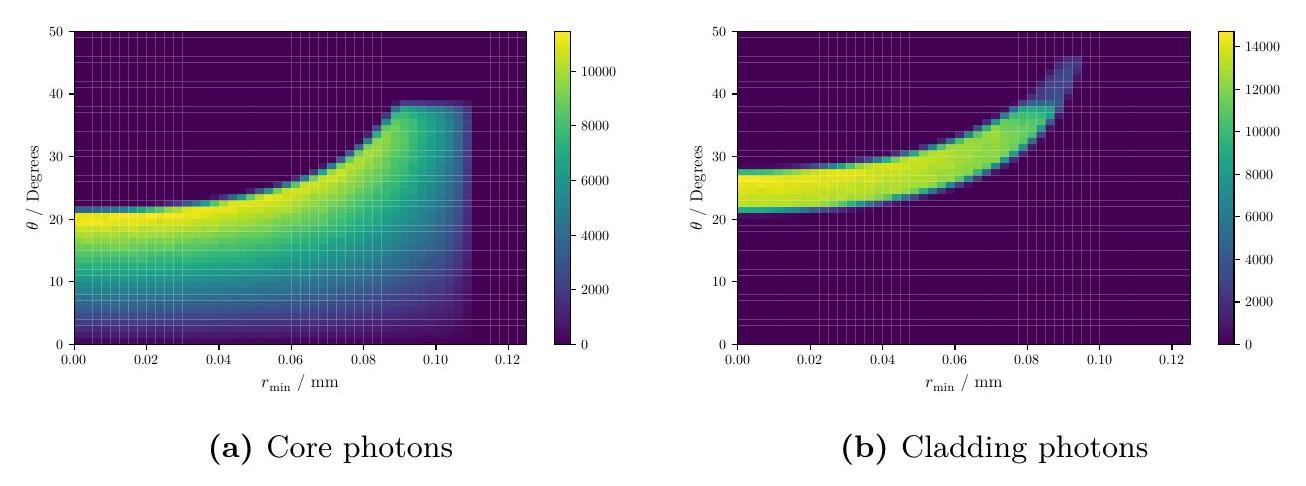
\includegraphics[max width=\textwidth, center]{2025_06_26_8f443d40fa1f5ba53fc3g-12(1)}

Figure 10: Two-dimensional histograms of the minimal distance $r_{\min }$ and angle $\theta$.\\
This distribution results from the fact that photons with $r_{\text {min }}>0$ values can experience total reflection even if their angle $\theta$ is larger than the already determined maximal angle.

This is explained by the effective angle between the photon and the cladding beeing lower then $\theta$ when the photon in not passing through the middle of the fiber.

\subsection*{5.3.4 Intensity}
The last study performed on the simulation samples focuses on the intensity relation described in (7). The aforementioned relation is visualized in Figure 11 using a twodimensional histogram of the angle $\theta$ and the gpsPosX variable ( $x$ position of the excitation in the fiber).\\
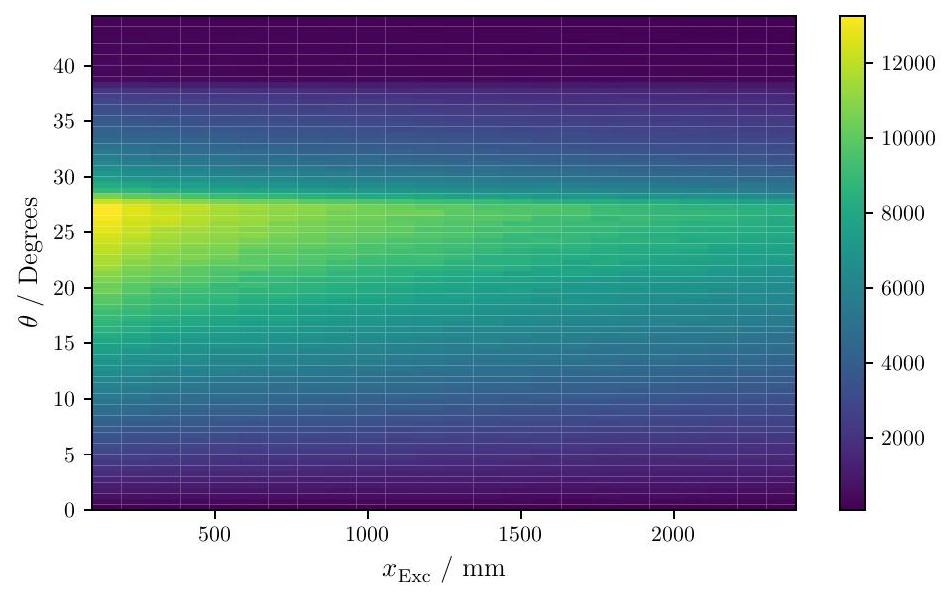
\includegraphics[max width=\textwidth, center]{2025_06_26_8f443d40fa1f5ba53fc3g-13}

Figure 11: Two-dimensional histogram of the intensity distribution in relation of the angle $\theta$ and the $x$ position of the excitation in the fiber.

Using the counts determined from the histogram, multiple fits of the intensity in relation to the gpsPosX variable are performed. As exlained in subsubsection 2.2.2, the intensity is described by (3), consequently the function


\begin{equation*}
I(x)=I_{0} \exp (-a x) \tag{8}
\end{equation*}


is used for the fits. A subsection of the detrmined fits for different horizontal angles is shown in Figure 12.\\
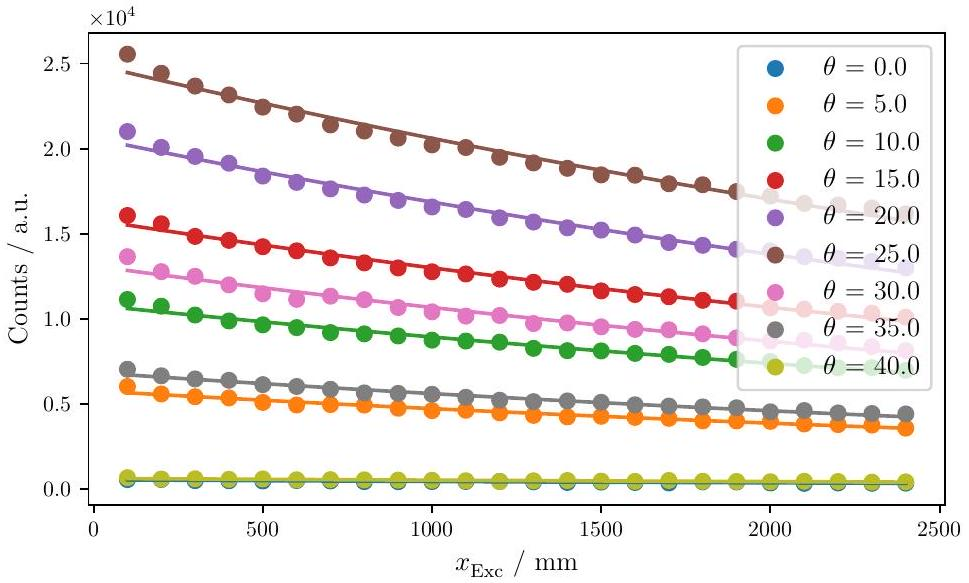
\includegraphics[max width=\textwidth, center]{2025_06_26_8f443d40fa1f5ba53fc3g-14(1)}

Figure 12: Fits on the determined intensities of the simulation samples against the gpsPosX variable at different angles $\theta$.

The determined fit parameter $a$ for each angle $\theta$ is then plotted in Figure 13 alongside the theoretical curve for $a_{\text {eff }}$ from (7).\\
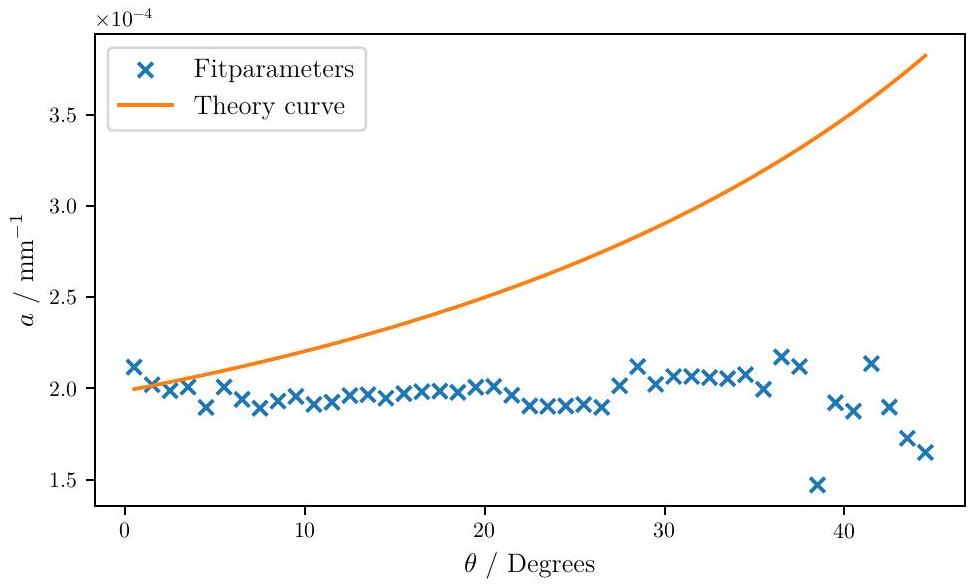
\includegraphics[max width=\textwidth, center]{2025_06_26_8f443d40fa1f5ba53fc3g-14}

Figure 13: The determined fit parameters $a$ with their respective angle and the expected curve.

\subsection*{5.4 Intensity measurement}
Similarly to the intensity fits for the simulation, the measured intensity is fitted against the gpsPosX variable. The determined fits are shown in Figure 14. Since the measurements don't follow the expected exponential slope, two fits per angle are performed and the mean of the fit parameter is used for further analysis.\\
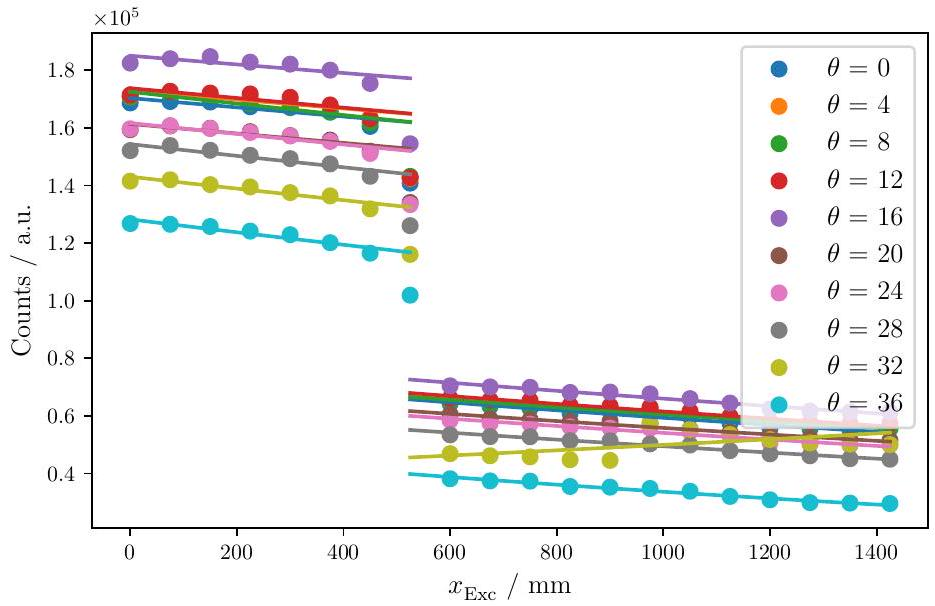
\includegraphics[max width=\textwidth, center]{2025_06_26_8f443d40fa1f5ba53fc3g-15(1)}

Figure 14: Fits on the measured intensities against the gpsPosX variable at different angles $\theta$.

The determined parameters $a$ are then again plotted against the angle $\theta$ in Figure 15. Using these parameters, another function of the form


\begin{equation*}
a(\theta)=\frac{A}{\cos (\theta)}+B \tan (\theta), \tag{9}
\end{equation*}


is fitted. The parameters and the corresponding fit are also shown in Figure 15\\
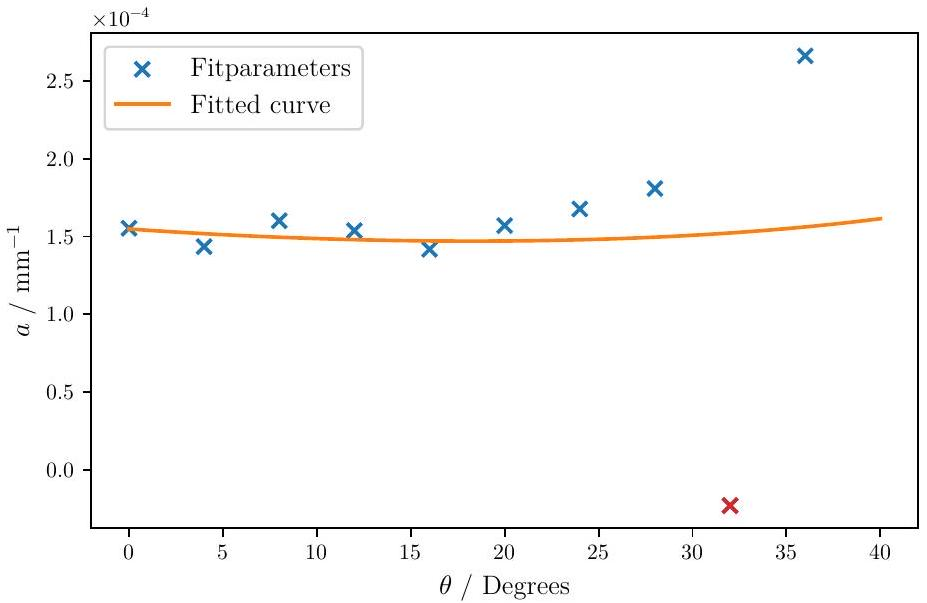
\includegraphics[max width=\textwidth, center]{2025_06_26_8f443d40fa1f5ba53fc3g-15}

Figure 15: Fit on the determined fit parameters $a$ against their respective angles $\theta$ and the outlier (red).

The data point marked red in Figure 15 lies far from the expected curve, so another fit without the outlier is performed in Figure 16.\\
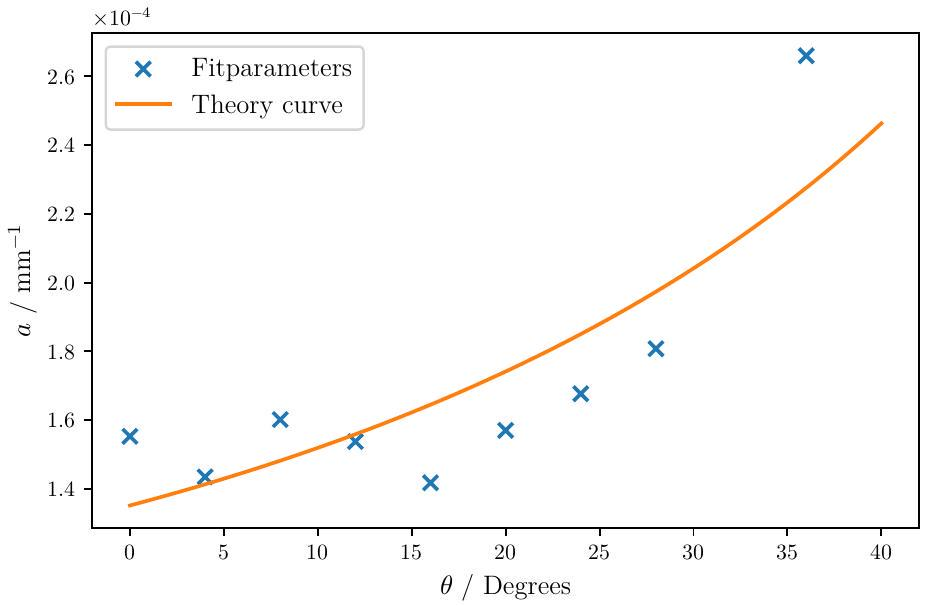
\includegraphics[max width=\textwidth, center]{2025_06_26_8f443d40fa1f5ba53fc3g-16}

Figure 16: Fit on the determined fit parameters $a$ against their respective angles $\theta$ with the outlier excluded.

The performed fits result in the parameters shown in Table 1.\\
Table 1: Comparison of fit parameters for (99 with and without the outlier.

\begin{center}
\begin{tabular}{ccc}
\hline
Parameter & Fit & Fit - Outlier excluded \\
\hline
$A$ & $(1.548 \pm 0.435) \times 10^{-4} 1 / \mathrm{m}$ & $(1.352 \pm 0.130) \times 10^{-4} 1 / \mathrm{m}$ \\
$B$ & $(-4.850 \pm 11.471) \times 10^{-5} 1 / \mathrm{m}$ & $(8.323 \pm 1.300) \times 10^{-5} 1 / \mathrm{m}$ \\
\hline
\end{tabular}
\end{center}

\subsection*{5.5 Angle Intensity Measurement}
For the final part of the analysis, the measured angle with the highest intensity is determined. The intensities for each angle are again calculated as the sum of the cleaned counts of each measurement. The angle determined to have the highest intensity is $\theta=29.5^{\circ}$. Both the angular distribution and the maximum angle are shown in Figure 17.\\
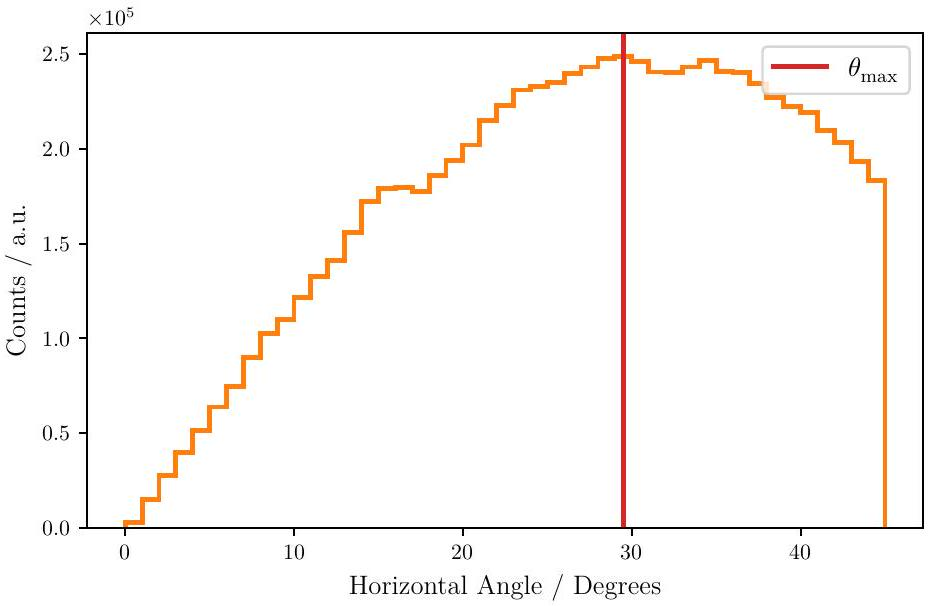
\includegraphics[max width=\textwidth, center]{2025_06_26_8f443d40fa1f5ba53fc3g-17}

Figure 17: Intensity distribution of the measured angle and the determined maximum angle.

\section*{6 Discussion}
The plots of the spectrum measurement show the effect of the roomlight very well. Also, the subtraction of the dark counts result in two very similar distributions. Only the measurement performed with the roomlight turned on shows some noise underlying the importance of a dark environment for the experiment.\\
When looking at Figure 7, the maximum intensity is expected at $0^{\circ}$ in both axes. In this case, the maximum is shifted by a few degrees, which may be attributed to a slightly misaligned fiber or measuring apparatus.\\
The maximum angles in the angular distribution shown in Figure 9 are in agreement with the calculated ones, showing only a minimal shift. The intensity seems to increase linearly with the angle until total reflection is reached. This is expected, as the reflected intensity is proportional to $\sin (\theta)$ because the photons are equally distributed in the solid angle. Thus for small angles, the sin will increase approximately linear.\\
Especially clean results can be observed in Figure 10. The distributions show that the cladding photons only have a distinct range in relation to their minimal distance and are cut off at an angle of about $21^{\circ}$. On the other hand, the core photons take over where no more cladding photons can be found, and allow for angles lower than the cladding ones. Additionally, Figure 10b shows the fact that a higher angle requires a higher $r_{\text {min }}$ value for the photon to still perform total reflection. This behavior is in good agreement with the expected result.\\
The first inconsistencies in the simulation samples can be observed during the determination of the angular dependence of the fit parameter $a$. For the simulation samples, the fit parameter shows no dependence on the angle. The explanation for this needs further information on the simulation method applied in the GEANT4 software. Due to this, no function was fitted on the obtained result in order to obtain a value on the minimal\\
distance.\\
A similar fit was performed on the measured samples leading to more meaningful results. Only one of the measurements resulted in an outlier. This outlier can be easily explained by a sudden jump in the intensity for $\theta=32^{\circ}$ in Figure 14. The origin of the jump may have resulted from a disturbance of the experimental setup during the measurement. Additionally, the drop in intensity shown in Figure 14 results from kink in the fiber at around 50 cm .\\
Lastly, the angular intensity measurement in Figure 17 shows no clear maximum. The maximum angle was determined as $29.5^{\circ}$, although this could also be a statistical fluctuation.

\section*{References}
[1] Lab Course E5a: Measurement of scintillating fibres for the LHCb experiment. TU Dortmund, Department of physics.


\end{document}